\PassOptionsToPackage{dvipsnames}{xcolor}
\documentclass{beamer}
%% \documentclass[aspectratio=169]{beamer}

\usepackage[latin1]{inputenc}

\usepackage{color}
%% \usepackage[dvipsnames]{xcolor}
%% \usepackage{amsmath}
%% \usepackage{amsfonts}

\usepackage{listings}
\lstset{
  language=C++,
  %% numbers=left,
  showstringspaces=false,
  formfeed=\newpage,
  tabsize=4,
  basicstyle=\footnotesize\ttfamily,
  commentstyle=\color{BrickRed}\itshape,
  keywordstyle=\color{blue},
  stringstyle=\color{OliveGreen}
  %% morekeywords={models, lambda, forms, dict, list, str, import, dir, help,
  %%  zip, with, open}
}

% Setup the tikz package for pictures.
\usepackage{tikz}
\usetikzlibrary{calc}
\usetikzlibrary{arrows}
\usetikzlibrary{shapes,decorations.pathmorphing}
\definecolor{theblue}{HTML}{236EAF}
\definecolor{theorange}{HTML}{F7800A}
\definecolor{thelightblue}{HTML}{98BBDA}
\definecolor{thedarkblue}{HTML}{02468F}
\tikzstyle{info}=[
  draw=thedarkblue,rectangle,rounded corners=1mm,inner sep=1mm,
  fill=theblue,ultra thick,text=white,font=\footnotesize
]
\tikzstyle{note}=[
  draw=BrickRed,rectangle,rounded corners=2mm,inner sep=3mm,
  fill=BrickRed,ultra thick,text=white,font=\footnotesize
]
\tikzstyle{noteline}=[
  draw=BrickRed,ultra thick
]
\tikzstyle{infoline}=[
  ultra thick,->
]
\tikzstyle{box}=[
  ultra thick
]
\tikzstyle{wow}=[
  ellipse,
  draw=red,
  ultra thick,
  fill=yellow,
  decoration=zigzag,
  decorate,
  font=\Huge,
  text width=0.6\textwidth,
  align=center,
  anchor=center,
  inner sep=1cm
]

% Set Beamer mode.
\mode<presentation>{
  \usetheme{Oxygen}
}

% Uncomment this if you need to eliminate the
% navigation icons on the bottom right.
%% \setbeamertemplate{navigation symbols}{}

\title[The Cut and Thrust of CUDA]{The Cut and Thrust of CUDA}
\author{Luke Hodkinson}
\institute{
  Center for Astrophysics and Supercomputing \\
  Swinburne University of Technology \\
  Melbourne, Hawthorn 32000, \underline{Australia}
}
\date{\today}

\begin{document}

\frame{\titlepage}

\frame{\frametitle{Table of contents}\tableofcontents}

\AtBeginSection[]
{
  \begin{frame}
    \tableofcontents[currentsection]
  \end{frame}
}

\section{Introduction}

\begin{frame}
  \frametitle{Purpose}
  A review of required C++ fundamentals.
  An introduction to thrust basics.
  Two successful case studies.
\end{frame}

\begin{frame}
  \frametitle{What is Thrust?}
  \begin{itemize}
    \item A parallel algorithms library.
    \item Resembles the C++ Standard Template Library.
    \item Enhances {\bf productivity}.
  \end{itemize}
  \hspace{5cm}
\includegraphics[width=3cm]{thrust_logo.png}
\end{frame}

\begin{frame}
  \frametitle{Architectures}
  Thrust is not limited to GPUs...
  \begin{columns}
    \begin{column}{.6\textwidth}
      \begin{itemize}
      \item Multicore CPUs.
      \item GPUs.
      \item CUDA.
      \item OpenMP.
      \item Intel Threading Building Blocks.
      \end{itemize}
    \end{column}
    \begin{column}{.4\textwidth}
      
\includegraphics[width=.38\textwidth]{cuda_logo.jpg} \\
      \vspace{.2cm}
      
\includegraphics[width=.38\textwidth]{tbb_logo.png} \\
      \vspace{.5cm}
      
\includegraphics[width=.38\textwidth]{openmp_logo.jpg}
    \end{column}
  \end{columns}
\end{frame}

\begin{frame}
  \frametitle{Current Statuts}
  \begin{itemize}
    \item Open source.
    \item Apache License 2.0.
    \item Version 1.6.0.
    \item Actively developed.
    \item 240+ active users.
    \item Now distributed with CUDA toolkit.
  \end{itemize}
\end{frame}

\section{Results}

\begin{frame}
  \frametitle{Results}
  \framesubtitle{The target problem}
  \begin{itemize}
    \item Conversion of an MPI parallel selection algorithm.
    \item Used to find median of large distributed arrays.
    \item Running with 10,000,000 elements per process.
    \item Written in C++ using generic algorithms (STL).
  \end{itemize}
\end{frame}

\begin{frame}
  \frametitle{Results}
  \framesubtitle{Programming effort}
  \begin{block}{Number of characters modified}
    \centering
    \vspace{1cm}
    {\Huge $24^*$}
    \vspace{1cm}
  \end{block}
  $^*$ {\it Not including build scripts or including headers.}
\end{frame}

\begin{frame}
  \frametitle{Results}
  \framesubtitle{Programming time}
  \begin{block}{Time spent modifying algorithm}
    \centering
    \vspace{1cm}
    {\Huge $\approx 1$ minute$^*$}
    \vspace{1cm}
  \end{block}
  $^*$ {\it Not including build scripts.}
\end{frame}

\begin{frame}
  \frametitle{Results}
  \framesubtitle{Speedup}
  \begin{block}{Measured speedup}
    \centering
    \vspace{1cm}
    {\Huge $122x^*$}
    \vspace{1cm}
  \end{block}
  $^*$ {\it Measured on gSTAR.}
\end{frame}

\begin{frame}
  \frametitle{Results}
  \framesubtitle{Scaling}
  \begin{center}
    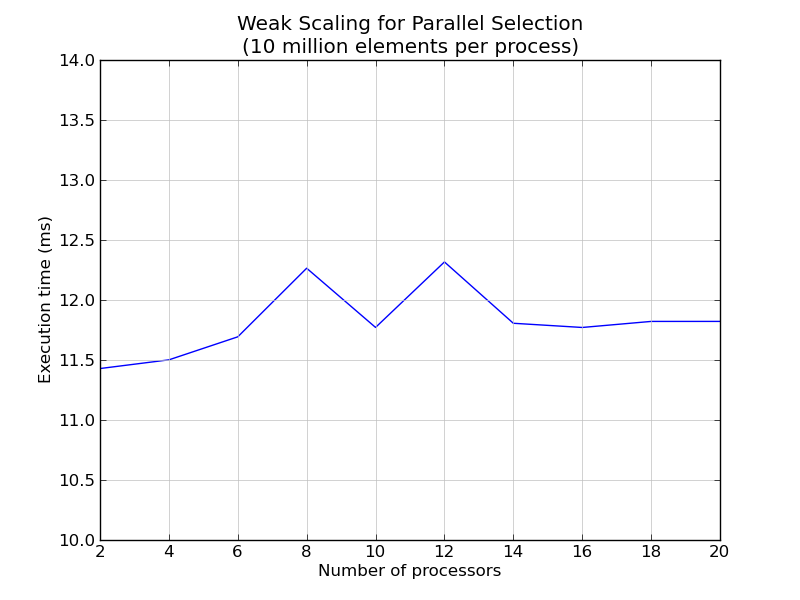
\includegraphics[width=.8\textwidth]{weak.png}
  \end{center}
\end{frame}

\begin{frame}
  \frametitle{Results}
  \framesubtitle{Metrics}
  \begin{block}{Metrics}
    \vspace{1cm}
    \hspace{0.5cm}{\Huge $x5$ per character changed.} \\
    \hspace{0.5cm}{\Huge $x2$ per second spent.}
    \vspace{1cm}
  \end{block}
\end{frame}

\begin{frame}
  \frametitle{Results}
  \framesubtitle{Metrics}
  \begin{center}
    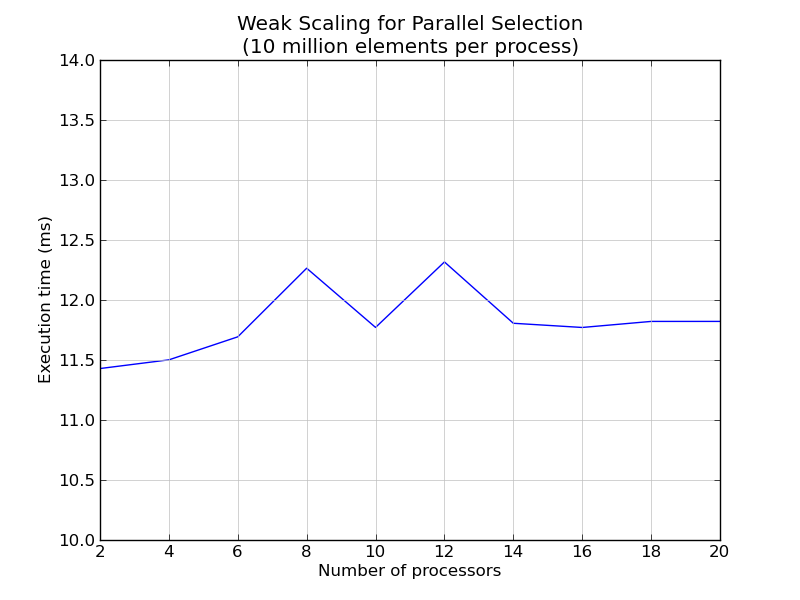
\includegraphics[width=.8\textwidth]{weak.png}
  \end{center}
  \visible<2>{
    \begin{tikzpicture}[remember picture,overlay]
      \pgftransformshift{\pgfpointanchor{current page}{center}}
      \node[wow,text width=4cm] at (0,0) {NOT \\REALLY};
    \end{tikzpicture}
  }
\end{frame}

\begin{frame}
  \frametitle{Results}
  {\Huge Of course...} \\
  \vspace{.5cm}
  \begin{itemize}
    \item results may vary,
    \item already written in C++,
  \end{itemize}
  \vspace{.5cm}
  which brings us to ...
\end{frame}

\section{C++ and Generics}

\begin{frame}
  \frametitle{Why Am I Talking About C++?}
  Because Thrust is written in C++. \\
  \vspace{.2cm}
  \hspace{.5cm}Why? \\
  \vspace{.2cm}
  \hspace{1cm}Because C++
  \vspace{.1cm}
  \begin{itemize}
    \item allows object-oriented programming,
    \item allows generic programming,
    \item maintains high performance.
  \end{itemize}
\end{frame}

\begin{frame}
  \frametitle{Why Am I Talking About C++?}
  Often critcized as ``too much rope''...
  \begin{itemize}
    \item potentially hidden operations,
    \item not truly object oriented,
    \item steep learning curve.
  \end{itemize}
\end{frame}

\begin{frame}
  \frametitle{Why Am I Talking About C++?}
  Fortunately we only need to cover a relatively small
  amount.
\end{frame}

\begin{frame}
  \frametitle{Object Oriented Programming}
  \framesubtitle{Why do we need it?}
  OO designs allow us to write customised CUDA kernels
  in optimised Thrust algorithms without having to
  actually write a kernel.
\end{frame}

\begin{frame}
  \frametitle{Object Oriented Programming}
  \framesubtitle{What is it?}
  A programming paradigm characterised by representation of concepts
  as ``objects'' that have both data and procedures which interact
  with one another.
  \begin{center}
    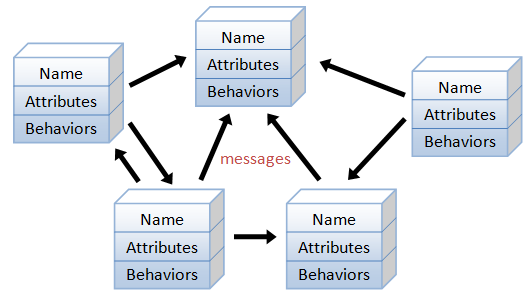
\includegraphics[width=.7\textwidth]{oop_objects.png}
  \end{center}
\end{frame}

\begin{frame}
  \frametitle{Object Oriented Programming}
  Some definitions:
  \begin{description}
    \item[class] A structure to hold data (members) and functions (methods).
    \item[object] An instantiaion of a class. Much like a struct, a class
      defines an object, but no allocation is given until instantiation.
  \end{description}
\end{frame}

\begin{frame}[fragile]
  \frametitle{Object Oriented Programming}
  Defining a class:
  \begin{example}
    \begin{columns}
      \begin{column}{.3\textwidth}
        \begin{lstlisting}
struct point_type {
  double x, y;
};
        \end{lstlisting}
      \end{column}
      \hspace{-10pt}
      \vrule{}
      \hspace{8pt}
      \begin{column}{.5\textwidth}
        \begin{lstlisting}
struct point_type {
  double x, y;

  double norm() {
    return sqrt(x*x + y*y);
  }
};
        \end{lstlisting}
      \end{column}
    \end{columns}
  \end{example}
\end{frame}

\begin{frame}[fragile]
  \frametitle{Object Oriented Programming}
  Instantiating a class into an object:
  \begin{example}
    \begin{lstlisting}
int main() {

  // Make an object of type "point_type".
  point_type point;

  // Call the "norm" method.
  double value = point.norm();

}
    \end{lstlisting}
  \end{example}
\end{frame}

\begin{frame}[fragile]
  \frametitle{Object Oriented Programming}
  \begin{itemize}
    \item Typically use \lstinline|class| instead of \lstinline|struct| (why?).
    \item Data members are automatically accessible to methods.
    \item Methods callable from objects using ``.''.
  \end{itemize}
\end{frame}

\begin{frame}[fragile]
  \frametitle{Object Oriented Programming}
  \framesubtitle{Functors}
  C++ allows certain operators to be ``overloaded''. \\
  \vspace{.5cm}
  \begin{center}
  \begin{tabular}{c|c}
    \lstinline|x + y| & \lstinline|point_type& operator+( const point_type& y )| \\
    \lstinline|x - y| & \lstinline|point_type& operator-( const point_type& y)| \\
    \lstinline|x*y| & \lstinline|point_type& operator*( const point_type& y )| \\
    \lstinline|x/y| & \lstinline|point_type& operator/( const point_type& y)| \\
    \hline
    \multicolumn{1}{|c|}{\lstinline|x()|} & \multicolumn{1}{c|}{\lstinline|void operator()()|} \\
    \hline
  \end{tabular}
  \end{center}
\end{frame}

\begin{frame}[fragile]
  \frametitle{Object Oriented Programming}
  \framesubtitle{Functors}
  So, we can make function-like objects (functors) with attached data...
  \begin{example}
    \begin{lstlisting}
    struct square_plus {
      double to_add;

      square_plus( double value )
        : to_add( value ) {}

      void
      operator()( double x ) {
        return x*x + to_add;
      }
    };
    \end{lstlisting}
  \end{example}
\end{frame}

\begin{frame}[fragile]
  \frametitle{Object Oriented Programming}
  \framesubtitle{Functors}
  \begin{example}
    \begin{lstlisting}
    int main() {

      square_plus op( 10 ); // create a "square_plus"
                            // object with "to_add"
                            // of 10

      op( 2 ); // call object, returns 40

      square_plus( 10 )( 2 ); // create and call

    }
    \end{lstlisting}
  \end{example}
\end{frame}

\begin{frame}
  \frametitle{Object Oriented Programming}
  \framesubtitle{Summary}
  \begin{block}{Summary}
  \begin{itemize}
    \item Bind data with functions using classes/objects.
    \item Initialize objects with constructors.
    \item Finalize objects with destructors.
    \item Create function-like objects with operator overloading.
  \end{itemize}
  \end{block}
\end{frame}

\begin{frame}[fragile]
  \frametitle{Object Oriented Programming}
  Object oriented concepts we won't be looking at:
  \begin{itemize}
    \item inheritance,
    \item polymorphism,
    \item encapsulation,
    \item dynamic dispatch.
  \end{itemize}
  \vspace{.5cm}
  \emph{There's a lot more to it!}
\end{frame}

\begin{frame}
  \frametitle{What is Generic Programming?}
  \framesubtitle{Some quotes}
  \begin{block}{}
  {\Large Generic programming is a paradigm for developing efficient, reusable
    software libraries.}
  \end{block}
\end{frame}

\begin{frame}
  \frametitle{What is Generic Programming?}
  \framesubtitle{Some quotes}
  \begin{block}{}
    {\Large Generic programming is about generalizing software components
      so that they can be easily reused in a wide variety of situations.}
  \end{block}
\end{frame}

\begin{frame}
  \frametitle{What is Generic Programming?}
  \framesubtitle{Some quotes}
  \begin{block}{}
    {\Large Generic programming is a style of computer programming
      in which algorithms are written in terms of to-be-specified-later
      types that are then instantiated when needed for specific types
      provided as parameters.}
  \end{block}
\end{frame}

\begin{frame}[fragile]
  \frametitle{What is Generic Programming?}
  \framesubtitle{Example problem}
  \begin{example}
    \begin{lstlisting}
    // Sum a set of numbers.
    int sum( int array[], int size ) {
      int result = 0;
      for( unsigned ii = 0; ii < size; ++ii )
        result += array[ii];
      return result;
    }
    \end{lstlisting}
  \end{example}
\end{frame}

\begin{frame}
  \frametitle{What is Generic Programming?}
  \framesubtitle{Example problem}
  What about types other than int? \\
  Solutions:
  \begin{itemize}
  \item Write different versions for each type.
    \begin{itemize}
    \item Fast, but unmanageable.
    \end{itemize}
  \item Use pointers to generalise type.
    \begin{itemize}
    \item mallocs for ints?! Too slow.
    \item Lose type information.
    \end{itemize}
  \item {\bf Use generic programming.}
  \end{itemize}
\end{frame}

\begin{frame}[fragile]
  \frametitle{Templates}
  Templates are how C++ handles generic programming.
  \begin{example}
    \begin{lstlisting}
    // Sum a set of numbers.
    template< typename T >
    T sum( T array[], int size ) {
      T result = 0;
      for( unsigned ii = 0; ii < size; ++ii )
        result += array[ii];
      return result;
    }
    \end{lstlisting}
  \end{example}
\end{frame}

\begin{frame}[fragile]
  \frametitle{Templates}
  \begin{example}
    \begin{lstlisting}
    int main() {

      int array_of_ints[10];
      double array_of_doubles[10];
      // TODO: Initialise arrays.

      sum<int>( array_of_ints, 10 );
      sum<double>( array_of_doubles, 10 );

      sum( array_of_ints, 10 );
      sum( array_of_doubles, 10 );

    }
    \end{lstlisting}
  \end{example}
\end{frame}

\begin{frame}[fragile]
  \frametitle{Templates}
  \begin{example}
    \begin{lstlisting}
    int main() {

      int array_of_ints[10];
      double array_of_doubles[10];
      // TODO: Initialise arrays.

      sum<int>( array_of_ints, 10 );
      sum<double>( array_of_doubles, 10 );

      sum( array_of_ints, 10 );
      sum( array_of_doubles, 10 );

    }
    \end{lstlisting}
  \end{example}
\end{frame}

\begin{frame}[fragile]
  \frametitle{Iterators}
  What if we have a more complex data type? Say, a linked list?
\end{frame}

\begin{frame}[fragile]
  \frametitle{Algorithms}
  Bring together object oriented programming and generic programming.
  Make objects that perform algorithms and are container agnostic.
\end{frame}

\begin{frame}[fragile]
  \frametitle{Templates}
  \begin{block}{Summary}
    \begin{itemize}
    \item Give functions/objects variable types.
    \item Very efficient, different code for each type.
    \item Manageable code.
    \item Allows separation of data and algorithms.
    \end{itemize}
  \end{block}
\end{frame}


%% \begin{frame}
%%   \frametitle{Generic Programming}
%%   \framesubtitle{What and why?}
%%   Explain generally how generics can save us a lot
%%   of effort by generalising algorithms to various kinds
%%   of data structures. Separation of algorithms and data.
%% \end{frame}

%% \begin{frame}
%%   \frametitle{Generic Programming}
%%   \framesubtitle{Templates}
%%   Achieved in C++ using Templates.
%%   As an example, show the conversion from an entirely C
%%   implementation of a function to a C++ templated one.
%% \end{frame}

%% \begin{frame}
%%   \frametitle{Generic Programming}
%%   \framesubtitle{Data Abstraction and the STL}
%%   Show examples of a bunch of the STL containers and 
%%   algorithms.
%% \end{frame}

%% \begin{frame}
%%   \frametitle{Generic Programming}
%%   \framesubtitle{Iterators}
%%   Explain iterators.
%% \end{frame}

\begin{frame}
  \frametitle{Performance}
  \framesubtitle{Zero-overhead principle}
  {\Huge ``You pay for what you use.''}
\end{frame}

\begin{frame}
  \frametitle{Performance}
  \framesubtitle{The Poor Compiler}
  Explain that with templates most of the overhead is
  in the compilation phase. The runtime can be faster.
\end{frame}

\begin{frame}
  \frametitle{Performance}
  \framesubtitle{Code Bloat}
  Talk about this concern and how it doesn't exist.
\end{frame}

\section{Thrust}

\begin{frame}
  \frametitle{CUDA Generics}
  We talked about generic algorithms, what if we could drop in
  replacement algorithms to take advantage of available hardware?
  \begin{itemize}
    \item What here...
  \end{itemize}
\end{frame}

\begin{frame}[fragile]
  \frametitle{Thrust Namespace}
  Just like the STL is declared inside the \\
  \vspace{.5cm}\hspace{1cm}\lstinline|std|\vspace{.5cm} \\
  namespace, all thrust symbols are declared inside the \\
  \vspace{.5cm}\hspace{1cm}\lstinline|thrust|\vspace{.5cm} \\
  namespace.
\end{frame}

\begin{frame}[fragile]
  \frametitle{Thrust Vectors}
  Device memory is distinct from host memory. We need a special
  container class to refer to device memory:
  \begin{block}{Thrust vector declaration}
    \begin{lstlisting}
    template< typename T >
    class thrust::device_vector<T>;
    \end{lstlisting}
  \end{block}
\end{frame}

\begin{frame}[fragile]
  \frametitle{Thrust Vectors}
  Values can be easily transferred from host to device.
  \begin{example}
    \begin{lstlisting}
    std::vector<float> host_vec( 100 );
    thrust::device_vector<float> dev_vec( 100 );
    thrust::copy( host_vec.begin(), host_vec.end(), dev_vec.begin() );
    \end{lstlisting}
  \end{example}
  Do a bit on noticing I left off the <float> in copy.
\end{frame}

\begin{frame}
  \frametitle{Thrust Algorithms}
  What kinds of algorithms can be optimised for multicore hardware?
  \begin{itemize}
    \item Transformation,
    \item reduction,
    \item sorting,
    \item and others.
  \end{itemize}
\end{frame}

\begin{frame}[fragile]
  \frametitle{Transformation}
  Apply a unary operation to each element of a vector and store the
  result in another (or the same) vector.
  \begin{center}
  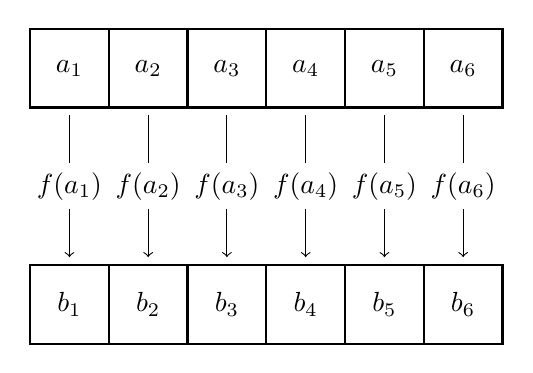
\begin{tikzpicture}[
      box/.style={thick},
      op/.style={rectangle,fill=white},
    ]
    \draw[box] (0,0) rectangle(6,1);
    \draw[box] (0,3) rectangle(6,4);
    \foreach \x in {1,...,6}{
      \draw[box] (\x,0) -- (\x,1);
      \draw[box] (\x,3) -- (\x,4);
      \draw[<-] (\x-.5,1.1) -- (\x-.5,2.9);
      \node at (\x-.5,0.5) {$b_\x$};
      \node at (\x-.5,3.5) {$a_\x$};
      \node[op] at (\x-.5,2) {$f(a_\x)$};
    };
  \end{tikzpicture}
  \end{center}
\end{frame}

\begin{frame}[fragile]
  \frametitle{Reduction}
  Apply a binary operation to successive elements of a vector and return
  the scalar result.
  \begin{center}
  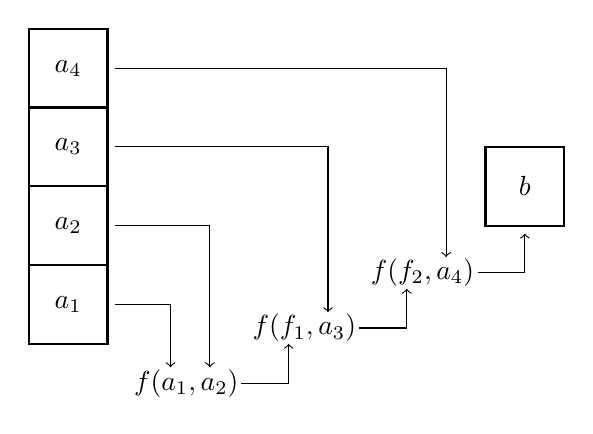
\begin{tikzpicture}[
      box/.style={thick},
      op/.style={rectangle,fill=white},
    ]
    \draw[box] (0,0) rectangle(1,4);
    \foreach \y in {1,...,4}{
      \draw[box] (0,\y) -- (1,\y);
      \node at (.5,\y-.5) {$a_\y$};
    };
    \node at (2,-.5) {$f(a_1,a_2)$};
    \node at (3.5,.2) {$f(f_1,a_3)$};
    \node at (5,.9) {$f(f_2,a_4)$};
    \draw[->] (1.1,.5) -- (1.8,.5) -- (1.8,-.3);
    \draw[->] (1.1,1.5) -- (2.3,1.5) -- (2.3,-.3);
    \draw[->] (1.1,2.5) -- (3.8,2.5) -- (3.8,.4);
    \draw[->] (1.1,3.5) -- (5.3,3.5) -- (5.3,1.1);
    \draw[->] (2.7,-.5) -- (3.3,-.5) -- (3.3,0);
    \draw[->] (4.2,.2) -- (4.8,.2) -- (4.8,.7);
    \draw[->] (5.7,.9) -- (6.3,.9) -- (6.3,1.4);
    \draw[box] (5.8,1.5) rectangle(6.8,2.5);
    \node at (6.3,2) {$b$};
  \end{tikzpicture}
  \end{center}
\end{frame}

\begin{frame}[fragile]
  \frametitle{Sorting}
  Apply an ordering to a vector.
\end{frame}

\begin{frame}
  \frametitle{M}
  Explain that the general operations, transformation and
  reduce, can be applied to a wide range of algorithms.
  Not all, but a wide range. Talk about how the internals of
  these general operations can be modified with functors.
\end{frame}

\begin{frame}[fragile]
  \frametitle{Advanced Iterators}
  Talk a little about \lstinline|constant_iterator|,
  \lstinline|counting_iterator|, \lstinline|transform_iterator| and
  \lstinline|zip_iterator|.
\end{frame}

\begin{frame}
  \frametitle{Examples of Uses}
  List all the different algorithms in the Thrust examples.
\end{frame}


\section{Case Studies}

\begin{frame}
  \frametitle{Distributed Median}
  \begin{itemize}
    \item In serial median can be calculated fairly
  easily by sorting the array and taking
  the $\frac{n}{2}$ element.
  \item With distributed array is considerable harder.
  \end{itemize}
\end{frame}

\begin{frame}
  \frametitle{Distributed Median}
  Define a balance function,
  \[ b(x) = N_l(x) - \frac{n}{2} \]
  which represents how close we are to the median by
  \[ b(x) = 0 \; . \]
  Here $N_l(x)$ is a count of how many elements are below the point $x$
  and $n$ is the number of elements in the array.
\end{frame}

\begin{frame}
  \frametitle{Distributed Median}
  Now we just need to find where $b(x) = 0$. We can do
  this with any root finder, but the Ridders algorithm
  will work particularaly well for us.
\end{frame}

\begin{frame}[fragile]
  \frametitle{Distributed Median}
  And already had one written.
  \begin{example}
    \begin{lstlisting}
    template< class Function,
              class T >
    T
    ridders( Function func,
             T x1,
	     T x2 );
    \end{lstlisting}
  \end{example}
\end{frame}

\begin{frame}[fragile]
  \frametitle{Distributed Median}
  \begin{example}
    \begin{lstlisting}[basicstyle=\tiny\ttfamily]
    template< typename Iterator >
    struct median_function
    {
      Iterator start, finish;
      long position;
      mpi::comm comm;

      long
      operator()( const value_type& x )
      {
        long sum_left = std::count_if(
          start, finish,
          std::bind2nd(
            std::less<value_type>(), x
          )
        );
        return comm.all_reduce( sum_left ) - position;
      }
    };
    \end{lstlisting}
  \end{example}
\end{frame}

\begin{frame}[fragile]
  \frametitle{Distributed Median}
  \begin{example}
    \begin{lstlisting}[basicstyle=\tiny\ttfamily]
    template< typename Iterator >
    struct median_function
    {
      long position;
      mpi::comm comm;

      __device__
      long
      operator()( const value_type& x )
      {
        long sum_left = thrust::count_if(
          start, finish,
          thrust::bind2nd(
            thrust::less<value_type>(), x
          )
        );
        return comm.all_reduce( sum_left ) - position;
      }
    };
    \end{lstlisting}
  \end{example}
\end{frame}

\begin{frame}[fragile]
  \frametitle{Distributed Median}
  \begin{example}
    \begin{lstlisting}
    int main() {
      thrust::device_vector<float> vec( 1000 );
      thrust::generate(
        vec.begin(), vec.end(),
        thrust::counting_iterator<float>( 0 )
      );
      float median = ridders(
        median_function<float>( start, finish ),
        0, 1000
      );
    }
    \end{lstlisting}
  \end{example}
\end{frame}


\begin{frame}
  \frametitle{Lattice Monte-Carlo Simulation}
  Courtesy of Michael Wang.
\end{frame}

%% \section{Conclusion}

%% \begin{frame}
%%   \frametitle{Bang for Buck}
%%   %% \framesubtitle{Some?}
%%   %% \begin{itemize}
%%   %%   \item 
%%   %% \end{itemize}
%%   Some algorithms are as good as custom kernels.
%% \end{frame}

%% \begin{frame}
%%   \frametitle{Generic Programming}
%%   %% \framesubtitle{Some?}
%%   %% \begin{itemize}
%%   %%   \item 
%%   %% \end{itemize}
%%   It's a big plus (plus).
%% \end{frame}

%% \begin{frame}
%%   \frametitle{Long Term Support}
%%   %% \framesubtitle{Some?}
%%   %% \begin{itemize}
%%   %%   \item 
%%   %% \end{itemize}
%%   Thrust included with CUDA now.
%% \end{frame}

\end{document}
